\documentclass[11pt]{article}
\usepackage[margin=1in]{geometry}
\usepackage{lmodern}
\usepackage[T1]{fontenc}
\usepackage{microtype}
\usepackage{graphicx}
\usepackage{booktabs}
\usepackage{multirow}
\usepackage{array}
\usepackage{xcolor}
\usepackage{listings}
\usepackage{tikz}
\usetikzlibrary{arrows.meta,positioning,shapes.misc,fit,backgrounds}
\usepackage[numbers,sort&compress]{natbib}
\usepackage[hidelinks]{hyperref}
\usepackage{caption}
\usepackage{enumitem}
\setlist{nosep,leftmargin=*}
\captionsetup{font=small,labelfont=bf}

\lstset{basicstyle=\ttfamily\footnotesize,breaklines=true,columns=fullflexible,frame=single,framerule=0.3pt,
  keepspaces=true,showstringspaces=false,xleftmargin=4pt,aboveskip=4pt,belowskip=4pt}

\newcommand{\sys}{Reels-RSI}
\newcommand{\todo}[1]{\textcolor{red}{[#1]}}

\title{\textbf{The Reel Is a Program:}\\[2pt]
\large Program-Level Self-Improvement for Code-Rendered Explainer Videos}

\author{%
\begin{tabular}{@{}c@{}}
\raisebox{-0.45\height}{
\includegraphics[height=1.15cm]{figures/alx-logo-crop.png}}\hspace{0.6em}%
\begin{tabular}[c]{@{}l@{}}\large\textbf{Agentic Loops X}\\[1pt]
\small Experiments in recursive intelligence\\[-1pt]
\small\url{https://github.com/agentic-loops-x}\end{tabular}
\end{tabular}
}
\date{\small October 2026 \quad\textbullet\quad Preprint \quad\textbullet\quad Code, rules, lessons and evolve report: \url{https://github.com/agentic-loops-x/Reels-RSI}}

\begin{document}
\maketitle

\begin{abstract}
Explainer videos---a worked geometry problem, why the sky is blue, how a dynasty fell---are usually
treated as one more target for pixel video generation. We argue they are a different modality: a
\emph{program} (a narration script, a storyboard and per-frame animation code) that a deterministic
renderer turns into frames. A program can be read, diffed and checked; pixels can only be watched.
We build on this with \sys{}, an open-source director that any agent harness can run, and with a
form of self-improvement that happens at the program level rather than in weights or prompts.
Every revision pass of a reel is logged with a code snapshot; a retrospective pairs each check
finding with the diff that fixed it and proposes lessons; a lesson that a static check can catch is
\emph{compiled into a rule} that ships with a must-fail and a must-pass example, so the memory itself
is unit-tested. Because reels are programs, a new rule can also be run backwards over everything the
system made before it learned the rule. A bounded, benchmark-gated step lets an agent rewrite the
director's playbook, kept only when blind pairwise judgments on held-out topics prefer it, and
every acceptance passes a human gate.
In a release-testing field study (23 reels, 136 frames, four languages, one skill-evolution round),
the one rule learned during the study found four latent defects in the 19 frames authored before it
existed and zero in the 117 authored under it; a skill rewrite that blind judges preferred 11--1 on
training topics and 8--4 on held-out topics left the absolute judge score unchanged
($75.3 \rightarrow 74.9$) and, on one history topic, dropped a fact the original stated. We document
three distinct ways the preference signal misled the loop and how program-level checks and human
gates caught them. Code, rules, lessons and the evolve report are public.
\end{abstract}

\section{Introduction}

A short explainer video has a peculiar property among media: nearly everything that matters in it
is \emph{symbolic}. The numbers in a worked problem, the labels on a map, the order of steps in a
derivation, the words the narrator says---these are the content, and the picture exists to deliver
them. Pixel-space video generators \citep{vbench2} are judged on whether motion looks plausible;
an explainer is judged on whether the triangle's area really is $0.3\,\mathrm{cm}^2$ and whether
the viewer saw why.

Recent systems therefore generate explainers as \emph{code}: Manim programs
\citep{theoremexplain2025,code2video2026,manimagent2026}, slide decks \citep{paper2video2025}, or
HTML compositions. Code gives exact text, real geometry and reproducible output. We take the
consequence one step further. If the reel is a program, then everything we know about programs
applies to reels: they can be linted, diffed, tested, audited retroactively, and ported between
the models that wrote them. In particular, an agent that makes reels can \emph{improve itself at
the program level}---by accumulating executable checks over its own output---instead of only in
its prompt or its weights.

This paper presents \sys{}, an open-source reel director, and the self-improvement loop built into
it. The system itself is engineering: a deterministic command-line pipeline (voice with per-word
timings, karaoke captions, font subsetting, procedural music and sound, maps, assembly, checks,
render) that any agent harness---Claude Code, Codex CLI, Gemini CLI, OpenCode---drives from a
Markdown skill; it makes reels in Chinese, English, Japanese, Korean, Spanish and French, and dubs
a finished reel into another language. The contribution we care about is what the program view
makes possible on top:

\begin{enumerate}
\item \textbf{A four-tier program-level memory} (\S\ref{sec:rsi}). Every finalize pass is logged
  with a code snapshot (L0). A retrospective pairs each check finding with the diff that fixed it
  and proposes \emph{lessons} that are injected into the next reel's frame briefs, scoped to the
  presets, aspects and modes they hold for (L1). A lesson that a static check can detect is
  \emph{compiled into a rule}---a \texttt{check(doc)} function shipped with a must-fail and a
  must-pass example, accepted only if it passes both (L2). A benchmark-gated step lets an agent
  rewrite the director's playbook, kept only if blind pairwise judges prefer the result on training
  \emph{and} held-out topics (L3). Nothing enters memory without a human \texttt{accept} or
  \texttt{apply}.
\item \textbf{Retroactive audit as a consequence of the program view} (\S\ref{sec:audit}). A rule
  learned from one reel is a program that can be run over every earlier reel. The rule learned
  during our study (\texttt{visible-from-state}) found four latent defects in two reels made before
  the system existed---defects no reviewer had noticed---and nothing in the 21 reels made under it.
\item \textbf{An honest account of the preference signal} (\S\ref{sec:evolve}). One
  skill-evolution round was accepted by blind pairwise judgment 11--1 on training topics and 8--4
  on held-out topics while the absolute 1--5 rubric score did not move. The judge-preferred
  version of one history reel also silently dropped a fact. We report three distinct failure
  modes of the preference signal observed in the study---a judge misreading that became a false
  lesson, a proposer writing an instruction aimed at the judge's sampling, and a craft-for-fact
  trade---and which gate caught each.
\end{enumerate}

We are explicit about scale: this is a field study of one system during its release testing (23
reels, one model family as director and judge, one evolution round), not a controlled benchmark.
A companion benchmark for explainer-reel systems with outcome tests on the final video is in
preparation and is deliberately kept out of this paper.

\section{Explainer reels as programs}
\label{sec:modality}

\paragraph{Definition.} In \sys{} a reel is a directory: \texttt{SCRIPT.md} (the spoken lines,
one per frame), \texttt{STORYBOARD.md} (per-frame scene, duration, transition, route, status),
one \texttt{.html} composition per frame under \texttt{compositions/frames/} (HTML, SVG, Canvas or Three.js, with
a single paused GSAP timeline), optional shared kits (\texttt{assets/*.js}) and overlays, and the
voice, caption and music assets the pipeline derives from them. Rendering is deterministic: a
headless browser seeks each composition's timeline to frame times and FFmpeg encodes
\citep{hyperframes}. Re-running \texttt{finalize} on a copy of a finished reel reproduces its
assembled composition byte for byte.

\paragraph{What the program view buys.} Table~\ref{tab:modality} contrasts the two routes to an
explainer video. The properties on the right are not claims about quality; they are what becomes
\emph{possible} once the artifact is source code.

\begin{table}[t]
\centering\small
\begin{tabular}{p{2.9cm}p{5.1cm}p{6.3cm}}
\toprule
& Pixel generation (Sora/Veo-style) & Program rendering (\sys{}, Manim-based agents) \\
\midrule
Text and numbers & sampled; may be wrong or illegible & exact strings in the program \\
Correctness check & watch the video (human or VLM) & read the program; render is deterministic \\
Targeted edit & regenerate & change one value, re-render one frame \\
Learning a mistake & fine-tune or re-prompt & write a check over the program text \\
Applying what was learned to old output & impossible & run the check over the corpus \\
Portability across models & none & the check is code, the model is irrelevant \\
Reproducibility & seed-dependent & byte-identical \\
\bottomrule
\end{tabular}
\caption{Two routes to an explainer video. The right column's properties are what \S\ref{sec:rsi}
builds on.}
\label{tab:modality}
\end{table}

\paragraph{Three layers of verification.} Because the artifact exists at three levels---program
text, assembled composition, rendered pixels---it can be checked at three levels with increasing
cost and decreasing certainty: \emph{static} rules over the program text (\S\ref{sec:rules}; exact,
free); \emph{dynamic} checks on the assembled composition (the renderer's own lint, runtime, layout
and contrast checks; exact for what they cover); and \emph{judged} assessment of sampled frames by a
vision-language model (cheap, informative, and---as \S\ref{sec:evolve} shows---not to be trusted
alone).

\section{\sys{}}
\label{sec:system}

\begin{figure}[t]
\centering
\resizebox{\textwidth}{!}{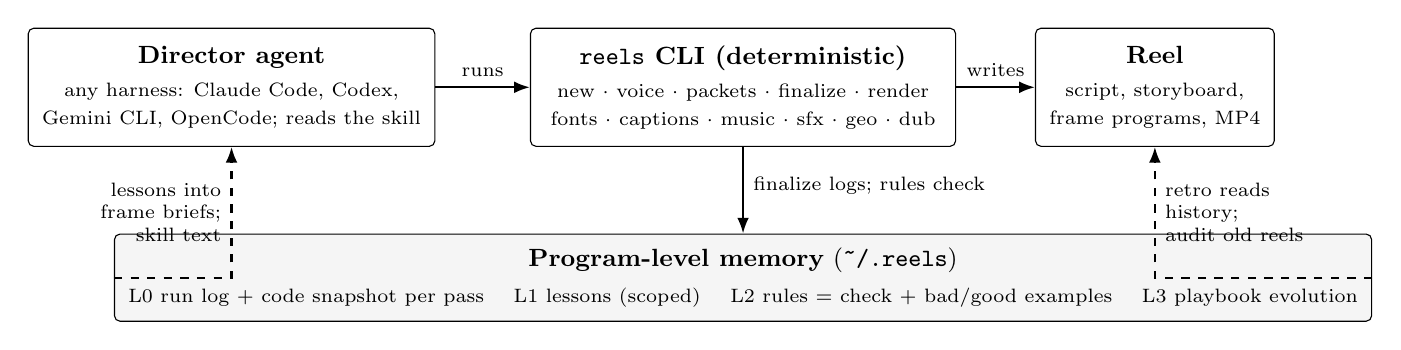
\begin{tikzpicture}[
  box/.style={draw,rounded corners=2pt,align=center,inner sep=5pt,font=\small},
  mem/.style={box,fill=black!4},
  arr/.style={-{Latex[length=2mm]},thick},
  feed/.style={-{Latex[length=2mm]},thick,dashed}]
\node[box,minimum width=4.2cm,minimum height=1.5cm] (agent) {\textbf{Director agent}\\[1pt]\scriptsize any harness: Claude Code, Codex,\\[-1pt]\scriptsize Gemini CLI, OpenCode; reads the skill};
\node[box,right=1.2cm of agent,minimum width=5.4cm,minimum height=1.5cm] (cli) {\textbf{\texttt{reels} CLI (deterministic)}\\[1pt]\scriptsize new $\cdot$ voice $\cdot$ packets $\cdot$ finalize $\cdot$ render\\[-1pt]\scriptsize fonts $\cdot$ captions $\cdot$ music $\cdot$ sfx $\cdot$ geo $\cdot$ dub};
\node[box,right=1.0cm of cli,minimum height=1.5cm] (reel) {\textbf{Reel}\\[1pt]\scriptsize script, storyboard,\\[-1pt]\scriptsize frame programs, MP4};
\node[mem,below=1.1cm of cli,minimum width=11.6cm] (mem) {\textbf{Program-level memory} (\texttt{\textasciitilde/.reels})\\[2pt]
\scriptsize L0 run log + code snapshot per pass \quad L1 lessons (scoped) \quad L2 rules = check + bad/good examples \quad L3 playbook evolution};
\draw[arr] (agent) -- node[above,font=\scriptsize]{runs} (cli);
\draw[arr] (cli) -- node[above,font=\scriptsize]{writes} (reel);
\draw[arr] (cli.south) -- node[right,font=\scriptsize,pos=.45]{finalize logs; rules check} (cli.south |- mem.north);
\draw[feed] (mem.west) -| node[left,font=\scriptsize,pos=.75,align=right]{lessons into\\frame briefs;\\skill text} (agent.south);
\draw[feed] (mem.east) -| node[right,font=\scriptsize,pos=.75,align=left]{retro reads\\history;\\audit old reels} (reel.south);
\end{tikzpicture}}
\caption{\sys{}. The creative half (script, storyboard, frame code, review) is the agent's; the
deterministic half is a CLI the agent calls. Memory sits beside both and is written only through
checks and human-gated acceptance.}
\label{fig:arch}
\end{figure}

\sys{} (Fig.~\ref{fig:arch}) separates the creative work from everything that must be
reproducible. The \textbf{skill} is 1{,}000 lines of Markdown---a ten-step director's handbook with
references for script and storyboard, frame construction, a quality bar, worked problems, history,
styles and techniques---that any file-reading, command-running agent can follow. The \textbf{CLI}
(5{,}000 lines of Python, standard library plus a TTS client and font tools) owns voice synthesis
with per-word timings, caption building with CJK-aware grouping and bilingual lines, font subsetting
so the headless renderer never shows missing glyphs, procedural music beds and sound effects cut to
the real narration, Natural Earth map layers, Wikimedia Commons images with credits, stroke-order
data for Chinese characters, assembly, overlays, transitions, the renderer's checks, snapshots and
render. Five visual presets (deep-space, notebook, ink, atlas, chalk) each ship a design spec, a
caption skin and, for chalk, a drawing kit.

\paragraph{Models are interchangeable at two seams.} The director runs inside whichever agent CLI
the user already has; \texttt{reels make "..."} launches a headless session. The judge and
retrospective roles are one-shot calls, \texttt{provider:model}, over an OpenAI-compatible or
Anthropic HTTP API or through a logged-in agent CLI; twelve providers plus custom endpoints are
configured in a TOML file. Nothing in memory depends on the model that produced it.

\paragraph{Languages.} A reel's language is detected from its script (Hangul, kana, Han, else
Latin with stop-word scoring); the voice, caption cutting (character-grouped for Chinese and
Japanese, word-grouped otherwise), glyph source (Noto SC/JP/KR, downloaded on first use) and
subtitle export follow. \texttt{reels dub} translates a finished reel's spoken lines and every
on-screen string in one model call, re-voices each line fitted to the original line's duration so
the frames stay in step, and re-renders; the geometry lesson of \S\ref{sec:study} exists in six
languages this way.

\section{Program-level self-improvement}
\label{sec:rsi}

The loop has four tiers. Each tier is written only by a check or by a person; the model proposes,
never commits.

\subsection{L0: every pass is evidence}
\texttt{reels finalize} assembles the reel and runs every check---the renderer's lint, runtime,
layout and contrast checks, then every \sys{} rule. Each pass appends a record to
\texttt{.reels/runs.jsonl} (findings with codes, lines and messages; frame count; duration) and
snapshots the frame sources to \texttt{.reels/history/NNN/}. Renders, scores and viewer feedback
(\texttt{reels feedback "the labels are too small" --frame 04}) append to the same log.

\subsection{L1: lessons, paired with the diff that earned them}
\texttt{reels retro} compiles an \emph{evidence file} from the log: per pass, which findings were
new and which were fixed; for every fixed finding, the unified diff between the snapshot where it
was present and the one where it was gone, labelled with what it fixed; the viewer's comments; the
judge's notes; and everything already known (accepted lessons and existing rules), so nothing is
proposed twice. A retrospective model reads the evidence and proposes at most five lessons, each
with a kind (\texttt{doc}, \texttt{rule}, \texttt{kit}, \texttt{taste}), a scope (director, frame,
solve, history, \ldots) and an optional \emph{when} condition (\texttt{preset=chalk},
\texttt{aspect=9:16}, \texttt{mode=solve}). Lessons land in an inbox. On \texttt{accept} they are
injected into the briefs of every future frame worker---but only the lessons whose conditions the
new reel satisfies, so a 16:9 science reel is not told how to draw chalk boxes on a portrait board.

\subsection{L2: a lesson that can be checked becomes a rule}
\label{sec:rules}
A rule is a directory: \texttt{rule.py} exposing \texttt{RULE} (id, severity, lesson, fix) and
\texttt{check(doc)} over a frame's text, plus \texttt{bad.*} files that must produce a finding and
\texttt{good.*} files that must not. \texttt{reels rules test} runs every rule against its examples;
\texttt{reels lessons accept --rule-dir} refuses a rule lesson whose rule fails them. Rules run on
every \texttt{finalize} and \texttt{lint}, so once accepted, the mistake cannot recur regardless of
which model is directing. Listing~\ref{lst:rule} shows the rule learned during the study; the rest
are listed in Appendix~\ref{app:rules}.

\begin{lstlisting}[language=Python,caption={The rule compiled from a lesson in the study. The must-fail example is the
original chalk-dust helper from the reel where the defect appeared; the must-pass example adds
\texttt{immediateRender:\ false} and a fade-in that is always safe.},label={lst:rule}]
RULE = {"id": "visible-from-state", "severity": "warning",
        "kinds": ["frame", "overlay", "kit"],
        "lesson": "fromTo renders its from-state at build time: a tween that starts "
                  "visible (opacity > 0) and fades to 0 later shows the element before its cue",
        "fix": "Add immediateRender: false to the to-vars"}

def check(doc):
    out = []
    for idx, args in H.calls(doc.text, "fromTo"):
        if len(args) < 4: continue                     # no position: starts at t=0 anyway
        frm, to = args[1], args[2]
        a, b = num(frm, "opacity"), num(to, "opacity")
        if a is not None and a > 0 and b == 0 and "immediateRender" not in to:
            out.append(H.Finding(RULE["id"], RULE["severity"], doc.rel,
                                 H.line_of(doc.text, idx),
                                 "fromTo starts visible and fades out - visible before its cue"))
    return out
\end{lstlisting}

The distinction between L1 and L2 is the distinction between advice and enforcement. A doc lesson
says ``labels inside coloured regions go at the region's widest part''; a model may or may not
follow it. A rule says ``a \texttt{fromTo} that starts visible and fades out without
\texttt{immediateRender:false} is a finding''; no model can skip it. Only mistakes that are
detectable from program text can become rules, which is a real limit (\S\ref{sec:limits}) and the
reason L1 exists.

\subsection{L3: the playbook rewrites itself, under a gate it cannot move}
\label{sec:evolve-method}
\texttt{reels evolve} runs one round: (1)~the current skill makes the four training topics of a
fixed eight-topic benchmark (science, history, worked problem, English); (2)~an agent reads the
baseline's judge notes, check findings and the lesson inbox and makes at most three edits to a
\emph{copy} of the skill's Markdown, explaining each in a changelog; (3)~the copy makes the same
topics; (4)~per topic, a vision judge sees both reels blind, three votes with the order swapped; the
candidate must win most votes, render at least as many reels, and lose no topic by more than ten
composite points; (5)~both versions make the four held-out topics and the candidate must win at
least half the votes there; (6)~a report with per-topic votes, the judge's reasons and a
side-by-side image of both reels is written, and nothing changes until a person runs
\texttt{evolve apply}. The proposer may edit only the skill text; the pipeline, the rules, the
presets, the judge's rubric and the benchmark topics are out of its reach, and it is told to write
tool defects it discovers into a separate file for a developer rather than working around them in
prose.

\section{Field study}
\label{sec:study}

\subsection{Setting}
The data are the reels \sys{} made during its own release testing, October 2026. Claude Code was the
director (Opus for the two reels made with a reviewer, Sonnet for the headless benchmark reels);
\texttt{claude-cli:sonnet} was the judge and the retrospective model. Table~\ref{tab:corpus} lists
the corpus. Two reels predate the system (made with its predecessor skill, before any rule existed);
two were made from scratch with a human reviewing at three gates (plan, look-dev, final); 17 were
made headlessly from one sentence each in the benchmark and evolve runs; two are dubs. A 30-second
headless reel cost \$0.56--1.29 and 230--584~s of wall time (15--34 agent turns); the judge takes
about 30~s per reel.

\begin{table}[t]
\centering\small
\begin{tabular}{lp{4.3cm}rrlp{3.4cm}}
\toprule
Group & Reels & Frames & Length & Lang. / aspect & Made by \\
\midrule
Pre-existing & 2 (Yuan dynasty; why the sky is blue) & 19 & 66--96 s & zh, 16:9 & predecessor skill, no rules \\
Reviewed & 2 (meeting problem; textbook geometry from a photo) & 16 & 55--84 s & zh, 9:16 & Opus, reviewer at 3 gates \\
Headless & 17 (8 topics $\times$ 2 skills, +1) & 83 & 26--33 s & zh/en, 16:9 & Sonnet, one sentence in \\
Dubbed & 2 (the geometry reel in en, ja) & 18 & 84 s & en, ja, 9:16 & \texttt{reels dub} \\
\midrule
Total & 23 & 136 & & 4 languages & \\
\bottomrule
\end{tabular}
\caption{The corpus. Dubs of the same reel into Spanish, French and Korean exist but were not rendered
at the time of writing and are excluded.}
\label{tab:corpus}
\end{table}

\subsection{Within a reel: the review loop converges}
Every reel reached zero check errors before render. The reviewed reels needed 7 and 5 finalize
passes; their warning counts went $5 \rightarrow 12 \rightarrow 2 \rightarrow 2 \rightarrow 1
\rightarrow 1 \rightarrow 1$ and $1 \rightarrow 1 \rightarrow 3 \rightarrow 2 \rightarrow 1$ (the rise
in pass 2 is new frames being added). The headless reels needed 1--6 passes (median 2); the hardest,
a history reel, went $3,4,3,0$ errors over four passes. Of the 13 reviewer interventions on the two
reviewed reels, 13 became fixes to the tool or the skill rather than to the reel alone, which is what
L1 is for.

\subsection{Lessons}
Retrospectives on the two reviewed reels and the agents' own retrospectives on the headless reels
produced 56 proposed lessons. A person accepted 15, rejected 1 and left 40 in the inbox (the inbox is
inert; nothing in it affects a reel). Of the 15: 12 are \texttt{doc} lessons (e.g.\ ``budget 3.9
Chinese characters per second for the teaching voice, not 4.5--5''; ``marks that underline a word
ride on the text element, never on guessed coordinates''), one is a \texttt{kit} lesson (every reel
gets a drawing kit; the chalk kit now ships with the preset), one is a \texttt{rule} lesson
(\S\ref{sec:audit}), and one \texttt{taste} lesson was reclassified. Two carry \emph{when}
conditions (\texttt{preset=chalk}, \texttt{aspect=9:16}); before conditions existed, a 16:9
deep-space reel was handed both.

The rejected lesson matters more than the accepted ones: the retrospective model had turned a
judge's note (``frame 09 is rendered at the wrong aspect, 1080$\times$640'') into ``verify every
frame's render dimensions before finalizing''. The frame was 1080$\times$1920; the judge had been
shown a sample sheet downscaled until each portrait frame was about 200 pixels wide. Had lessons
been accepted automatically, a false constraint would have reached every subsequent reel. The
retrospective prompt now ranks evidence (check findings and viewer words over judge notes) and the
sample sheets are sized per aspect.

\subsection{Lesson to rule, and the audit it enables}
\label{sec:audit}
In the first reviewed reel a chalk-dust puff showed stray specks before its cue. The cause is a GSAP
semantic: \texttt{fromTo} renders its from-state at build time, so a tween from opacity 0.9 to 0,
placed later in the timeline, shows the element from the first frame. The fix is one property. The
lesson became the rule of Listing~\ref{lst:rule}; its must-fail example is the original helper. We
then ran all 13 rules over the entire corpus (Table~\ref{tab:audit}).

\begin{table}[t]
\centering\small
\begin{tabular}{lrrrl}
\toprule
Reels & Frames & Authored & Findings & Where \\
\midrule
2 pre-existing & 19 & before the rule & 4 & Yuan: frames 06, 09, 11; sky: frame 04 \\
21 later & 117 & with the rule active & 0 & \\
\bottomrule
\end{tabular}
\caption{Retroactive audit with \texttt{visible-from-state}. The other 12 rules (ported from the
predecessor's checker, under which the pre-existing reels were made) produced no findings on any reel.}
\label{tab:audit}
\end{table}

All four findings are real by construction---each is a fade-out tween whose visible from-state
renders at $t=0$---and the sky reel's finding was confirmed in a rendered frame: a ripple ring that
should appear at its cue is already standing in the picture at 21.0~s. Two of the reels had been
delivered and reviewed by a person; nobody had noticed. This is the property Table~\ref{tab:modality}
promised: a lesson learned on reel $n$ is a program, and programs run on reels $1 \ldots n-1$. A
text lesson could not have found these; neither could a judge that was never asked.

The guard side of the same table is the zero: 117 frames authored under the rule contain no instance
of the pattern, although the agents that wrote them never saw the lesson in prose---the rule fires at
\texttt{finalize}, and the fix is one line.

\subsection{One evolution round}
\label{sec:evolve}
The round ran overnight on a consumer subscription, paused once for two hours when the quota ran out,
and resumed from its state file; 16 headless reels plus about 40 judge calls, \$12.75 in agent cost.
The proposer made three edits (59-line patch): checkable minimums for hero size and camera motion,
``mechanism recipes'' (show travel and effect, do not label them), and board legibility for worked
problems. It also traced a broken 16:9 board in a chalk reel to a hard-coded portrait canvas in the
shipped kit---a code defect, fixed by hand.

\begin{table}[t]
\centering\small
\begin{tabular}{lcc|cc}
\toprule
 & \multicolumn{2}{c|}{Absolute composite (0--100)} & \multicolumn{2}{c}{Blind pairwise votes} \\
 & baseline & candidate & baseline & candidate \\
\midrule
Train (4 topics) & 75.3 & 74.9 & 1 & \textbf{11} \\
Holdout (4 topics) & 72.8 & 73.5 & 4 & \textbf{8} \\
\bottomrule
\end{tabular}
\caption{The first evolve round. Composite $= 0.6 \cdot$ judge rubric $+ 0.4 \cdot$ deterministic
score; the deterministic part was at or near 100 for both, so the absolute column is the judge's
1--5 rubric. Every holdout topic split 2--1.}
\label{tab:evolve}
\end{table}

Table~\ref{tab:evolve} is the reason the verdict is pairwise. The same judge, asked for absolute
rubric scores, could not tell the versions apart; asked which of two reels on the same topic is
better, with the order swapped between votes, it preferred the candidate on 11 of 12 training votes
and 8 of 12 held-out votes. Fig.~\ref{fig:seasons} shows the largest change. The round was accepted
and, after inspection of the side-by-side images, applied by a person.

\begin{figure}[t]
\centering
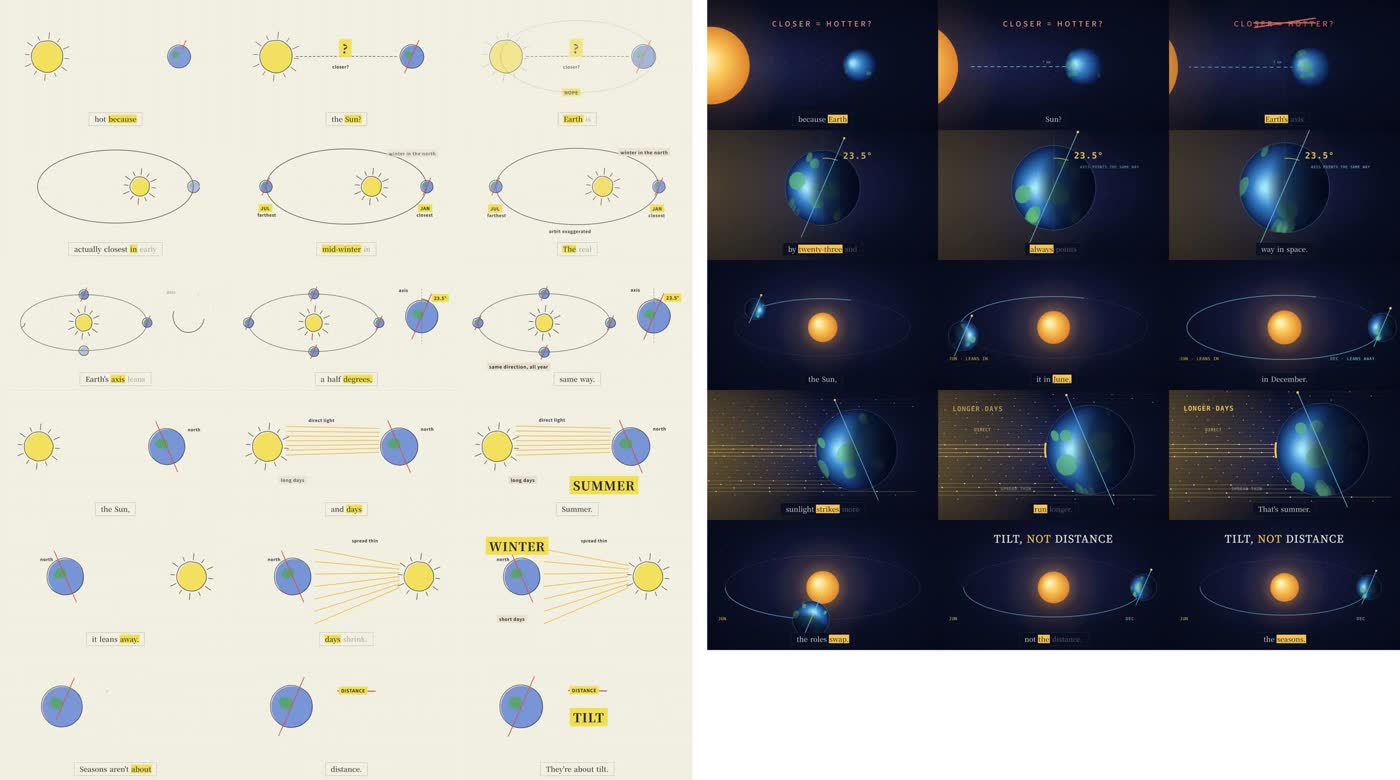
\includegraphics[width=\textwidth]{figures/evolve-seasons.jpg}
\caption{\emph{Why do we have seasons?} under the baseline skill (left) and the evolved skill
(right); same topic, same model, each row one frame sampled at 30/60/92\% of its duration. The judge
preferred the right 3--0.}
\label{fig:seasons}
\end{figure}

\subsection{Three ways the preference signal misled the loop}
\label{sec:hacking}
We record these because they happened, each was caught by a different gate, and a loop without that
gate would have absorbed them.

\paragraph{(a) A judge misreading became a proposed lesson.} Described above; caught at the human
\texttt{accept} gate, then prevented upstream by sizing the sample sheets and ranking evidence.

\paragraph{(b) The proposer wrote for the sampler.} One edit in the accepted patch read ``the
30/60/92\,\% samples must differ by camera position''---an instruction about the judge's sampling
schedule, not about what a viewer sees. Caught at the human \texttt{apply} gate and rewritten as
``keep the picture changing until the narration ends''; the proposer prompt now forbids instructions
aimed at sampling. This is the ``teaching to the test'' of \citet{notanoracle2026} in a creative
setting.

\paragraph{(c) Craft was bought with a fact.} On the Red Cliffs topic the candidate reel is visibly
richer (Fig.~\ref{fig:chibi}) and won 2--1. Its script lists three reasons Cao Cao lost and never
names the Sun--Liu alliance that beat him; the baseline devotes a frame to it. Nothing in the
evolve verdict looks at facts. The reel is a program, so the omission is a one-line \texttt{grep}
over \texttt{SCRIPT.md}---which is how we found it---but the loop did not run that grep, because no
rule asked for it. A rule cannot know which facts a topic requires; an outcome test can, which is
what the companion benchmark adds and why we keep it separate.

\begin{figure}[t]
\centering
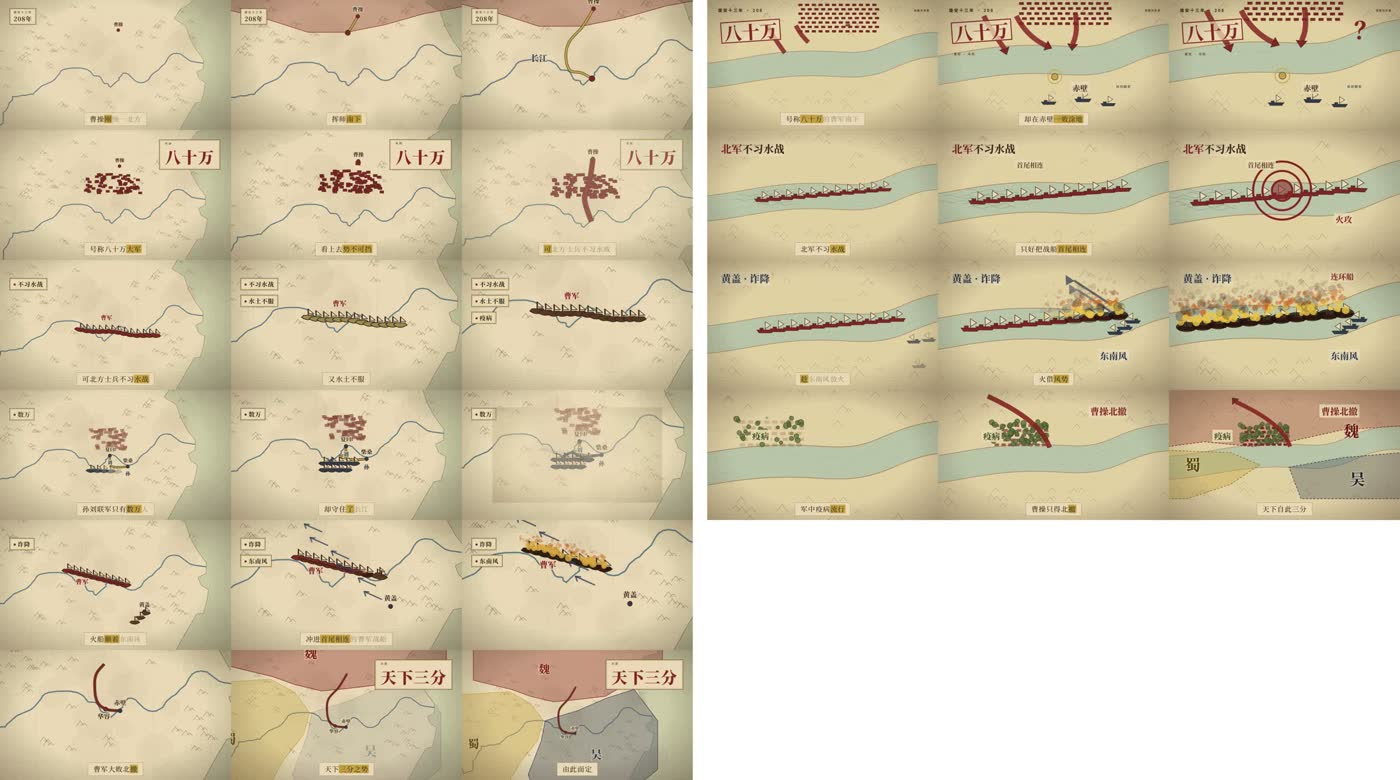
\includegraphics[width=\textwidth]{figures/evolve-chibi.jpg}
\caption{Red Cliffs, baseline (left) and evolved (right). The baseline's fourth row shows the
Sun--Liu alliance holding the river; the evolved reel has no such frame and its narration never names
the alliance. The judge preferred the right 2--1 for its larger, animated fire scene.}
\label{fig:chibi}
\end{figure}

Together with the flat absolute score, these support a conclusion others have reached in other
settings \citep{notanoracle2026,moreconvincing2026,teachingmonster2026}: a learned judge is a useful
\emph{advisor} to a self-improving loop and a poor \emph{oracle}. The program view lets the loop keep
its oracles deterministic---rules, render checks, and (in the benchmark) outcome tests on the
artifact---and reserve the judge for what only taste can rank.

\section{Related work}

\paragraph{Explainer and educational video from code.} TheoremExplainAgent \citep{theoremexplain2025}
and Code2Video \citep{code2video2026} generate Manim programs with planner/coder/critic agents and
judge them with LLM rubrics or a quiz; Paper2Video \citep{paper2video2025} adds pairwise ``arena''
comparison against human talks. ManimAgent \citep{manimagent2026} is closest to us: a Manim-writing
agent with an episodic memory of success rationales and validated failure patterns grown from its own
task stream, evaluated with blind human Pass@1. Its memory is prose retrieved into the prompt; ours
compiles the checkable part into tested code, which is what makes retroactive audit and cross-model
portability possible. CineForge \citep{cineforge2026} and VideoWeaver \citep{videoweaver2026} evolve
policies or skills for long-form pixel video; their learned knowledge cannot be run over the
artifact because the artifact is not a program.

\paragraph{Experience memory for agents.} Reflexion \citep{reflexion2023}, ExpeL \citep{expel2024}
and ACE \citep{ace2026} store verbal reflections, insights or an evolving playbook; our L1 and L3
belong to this family, with ACE's incremental playbook closest to \texttt{evolve}. Voyager
\citep{voyager2023} and ASI \citep{asi2025} store \emph{skills} as executable programs verified by
the environment; we store \emph{checks}, verified by their own examples, which is what a creative
task without an environment reward affords. The neuro-symbolic dual memory of
\citet{neurosymbolicmem2026} induces executable Python verifiers from failed trajectories and
validates them on positive and negative pools---the same idea as our L2 in a web and household
setting. SkillRevise \citep{skillrevise2026} revises LLM-authored skills from execution traces.

\paragraph{Checkers from fixes.} KNighter \citep{knighter2025} synthesises static analysers from
historical kernel patches, validating each against the buggy and the patched code, and found 92
long-latent Linux bugs; test-driven checker development \citep{codechecker2024} makes the same
contract explicit. Our rules follow this contract exactly---must-fail, must-pass---but the corpus
being audited is the agent's own past output, and the patches come from the agent's own revision log.

\paragraph{Self-modifying agents and judge reward hacking.} ADAS \citep{adas2024}, the Darwin G\"odel
Machine \citep{dgm2025} and GEPA \citep{gepa2025} let an agent rewrite its scaffold or prompts under
an objective score. \citet{notanoracle2026} and \citet{moreconvincing2026} show what happens when the
score is an LLM judge; \citet{fragility2026} shows how sensitive such loops are to variance and task
order. Our evolve step is a small instance of this family with the guards they recommend: a frozen
holdout, pairwise rather than absolute judgment \citep{mtbench2023}, a deterministic layer the proposer
cannot edit, and a person at the end.

\section{Limitations}
\label{sec:limits}
\emph{Scale.} 23 reels, one evolution round, one model family as director, judge and retrospective
model. The 11--1 and 8--4 votes are from one judge model; we have no human preference study, so we
cannot say whether the judge's taste matches viewers', only that it diverges from correctness.
\emph{What rules can see.} A rule checks program text; it cannot know that a topic requires naming an
alliance, that a label is too small for a phone, or that a mood is wrong. Those remain lessons
(advice) or outcome tests (the companion benchmark). \emph{Twelve of thirteen rules} were ported from
the predecessor's checker, each from a real failure, but only one rule's lesson-to-rule path was
exercised in this study. \emph{Dependencies.} The free neural voices come from an unofficial endpoint;
commercial use needs a licensed provider, which the pipeline supports. \emph{Judge saturation.} The
absolute rubric was flat across a change that pairwise judgment found decisive; we do not know how
much of the pairwise margin is the judge's position-independent taste and how much is noise, since each
topic was made once.

\section{Conclusion}
An explainer reel that is rendered from a program is a different object from a generated video, and
the difference is worth more than exact text: it makes the agent's own output something it can check,
audit and learn from at the level of code. \sys{} turns that into a loop---log, pair findings with
fixes, propose lessons, compile the checkable ones into tested rules, rewrite the playbook under a
gate---and a release-testing study shows each tier doing something a prose memory could not: a rule
found latent defects in reels made before it existed, scoped lessons stopped reaching reels they did
not fit, and three failures of the preference signal were each caught by a deterministic check or a
person before they entered memory. The system, every rule with its examples, the lessons and the
evolve report are public at \url{https://github.com/agentic-loops-x/Reels-RSI}.

\bibliographystyle{plainnat}
\bibliography{refs}

\appendix
\section{The thirteen rules}
\label{app:rules}
Each rule directory holds \texttt{rule.py}, at least one must-fail example and one must-pass example;
\texttt{reels rules test} passes 13/13. Severity \emph{error} blocks render; \emph{warning} is
reported.

\begin{table}[h]
\centering\small
\begin{tabular}{llp{9.6cm}}
\toprule
Rule & Severity & What it catches \\
\midrule
\texttt{timeline-registration} & error & a sub-composition that does not register its paused timeline under its composition id \\
\texttt{nondeterminism} & error & \texttt{Math.random}, \texttt{Date.now}, \texttt{requestAnimationFrame}, timers or self-driving animation in a seek-rendered frame \\
\texttt{cjk-font} & error & CJK text without an \texttt{@font-face} for a shipped font (the render browser has no CJK system fonts) \\
\texttt{dasharray-attr} & error & a \texttt{stroke-dasharray} attribute in the markup of a path that a tween draws on \\
\texttt{svgorigin-one-sided} & error & \texttt{svgOrigin} given only in a \texttt{fromTo}'s to-vars \\
\texttt{negative-zindex} & error & a negative z-index, which puts the layer behind the composition root \\
\texttt{caption-band} & warning & frame text placed in the band reserved for karaoke captions \\
\texttt{chained-no-position} & warning & a chained \texttt{.to()} without a position argument, which drifts to the timeline's end \\
\texttt{repeat-fromto} & warning & a second \texttt{fromTo} on the same target without \texttt{immediateRender:false} \\
\texttt{round-cap-mask} & warning & a reveal mask with round caps, which leaks a dot before the stroke begins \\
\texttt{polygon-winding} & warning & a counter-clockwise ring in d3-geo map data (``the globe minus this shape'') \\
\texttt{unpinned-cdn} & warning & a CDN script without a version pin \\
\texttt{visible-from-state} & warning & a \texttt{fromTo} that starts visible and fades out without \texttt{immediateRender:false} (learned in this study) \\
\bottomrule
\end{tabular}
\caption{Rules shipped with \sys{} 0.1. A user's own rules live beside them and may override a built-in of the same name.}
\end{table}

\section{Accepted lessons}
The 15 lessons a person accepted during the study, as injected into frame briefs (abridged).
\begin{itemize}
\item \textsc{frame} ---  A tween starting from a visible state on an element meant to appear later needs \texttt{immediateRender:false} (\emph{rule}).
\item \textsc{frame} ---  Labels inside coloured regions go at the region's widest part and get a board-coloured outline.
\item \textsc{frame} ---  Underlines, boxes and circles that mark a piece of text ride on the text element, never on guessed coordinates.
\item \textsc{frame} ---  Draw chalk boxes from four straight wobbly segments; curve-smoothing turns a rectangle into a blob (\emph{when preset=chalk}).
\item \textsc{frame} ---  On 9:16 canvases scale the hero to the full width and use the lower half for the working (\emph{when aspect=9:16}).
\item \textsc{frame} ---  Size on-figure labels at 28~px or larger; keep construction lines heavy and inside the figure.
\item \textsc{frame} ---  Pick label colours as pre-lightened variants that pass contrast on the board.
\item \textsc{frame} ---  Highlight a named composite shape by filling its parts, not by tracing a thin outline; put the answer box beside it.
\item \textsc{frame} ---  A hero word goes in an empty region of the hero, never over bright strokes.
\item \textsc{frame} ---  Clamp computed rays so endpoints and labels land inside the canvas above the caption band.
\item \textsc{director} ---  Budget about 3.9 characters/s for the female teaching voice and 4.5 for the male narrator; add 10\% when reading letter names.
\item \textsc{director} ---  Spread each frame's build-up across its narration; single out the key shape on the word that names it.
\item \textsc{solve} ---  Give every reel a drawing kit with the figure computed from coordinates (\emph{kit}).
\item \textsc{solve} ---  For a problem from a photo, transcribe text and figure, restate them for confirmation, and build the figure from the given lengths, never from pixel proportions.
\end{itemize}

\end{document}
